\section{Experimental results} \label{section:results}
We have implemented the algorithms in C++ and conducted the experiments
on Linux PCs with Intel Core i7 processor with 4 cores, enabling 8 threads
with the hyper threading technology. We have used the Graph-cuts
optimization code written by Veksler, using the libraries provided by
Boykov and Kolmogorov~\cite{middle_bury,2,3,4_below}.
% [2] Fast Approximate Energy Minimization via Graph Cuts.
%         Y. Boykov, O. Veksler, and R. Zabih.
%         In IEEE Transactions on Pattern Analysis and Machine Intelligence
%         (PAMI), vol. 23, no. 11, pages 1222-1239, November 2001.  
%
%     [3] What Energy Functions can be Minimized via Graph Cuts?
%         V. Kolmogorov and R. Zabih. 
%         In IEEE Transactions on Pattern Analysis and Machine Intelligence
%         (PAMI), vol. 26, no. 2, pages 147-159, February 2004. 
%         An earlier version appeared in European Conference on Computer
%         Vision (ECCV), May 2002.
%
%     [4] An Experimental Comparison of Min-Cut/Max-Flow Algorithms for
%         Energy Minimization in Vision. 
%         Y. Boykov and Vladimir Kolmogorov.
%         In IEEE Transactions on Pattern Analysis and Machine Intelligence
%         (PAMI), vol. 26, no. 9, pages 1124-1137, September 2004. 
We have used the QPBO and TRW-S implementations by
Kolmogorov~\cite{msr_link?,trw_link}.



The figure illustrates the convergence rate of three competing methods
(alpha expansion, parallel alpha expansion, hierarchical fusion) against
our swarm fusion method (only binary fusion without proposal
generation \chen{We generate proposals on the fly for optical flow and layered depth map. So the time actually includes proposal generation stage which can be ignored. I think we can just delete this sentence.}).

\hang{figure file missing}
\begin{figure}[tb]
%  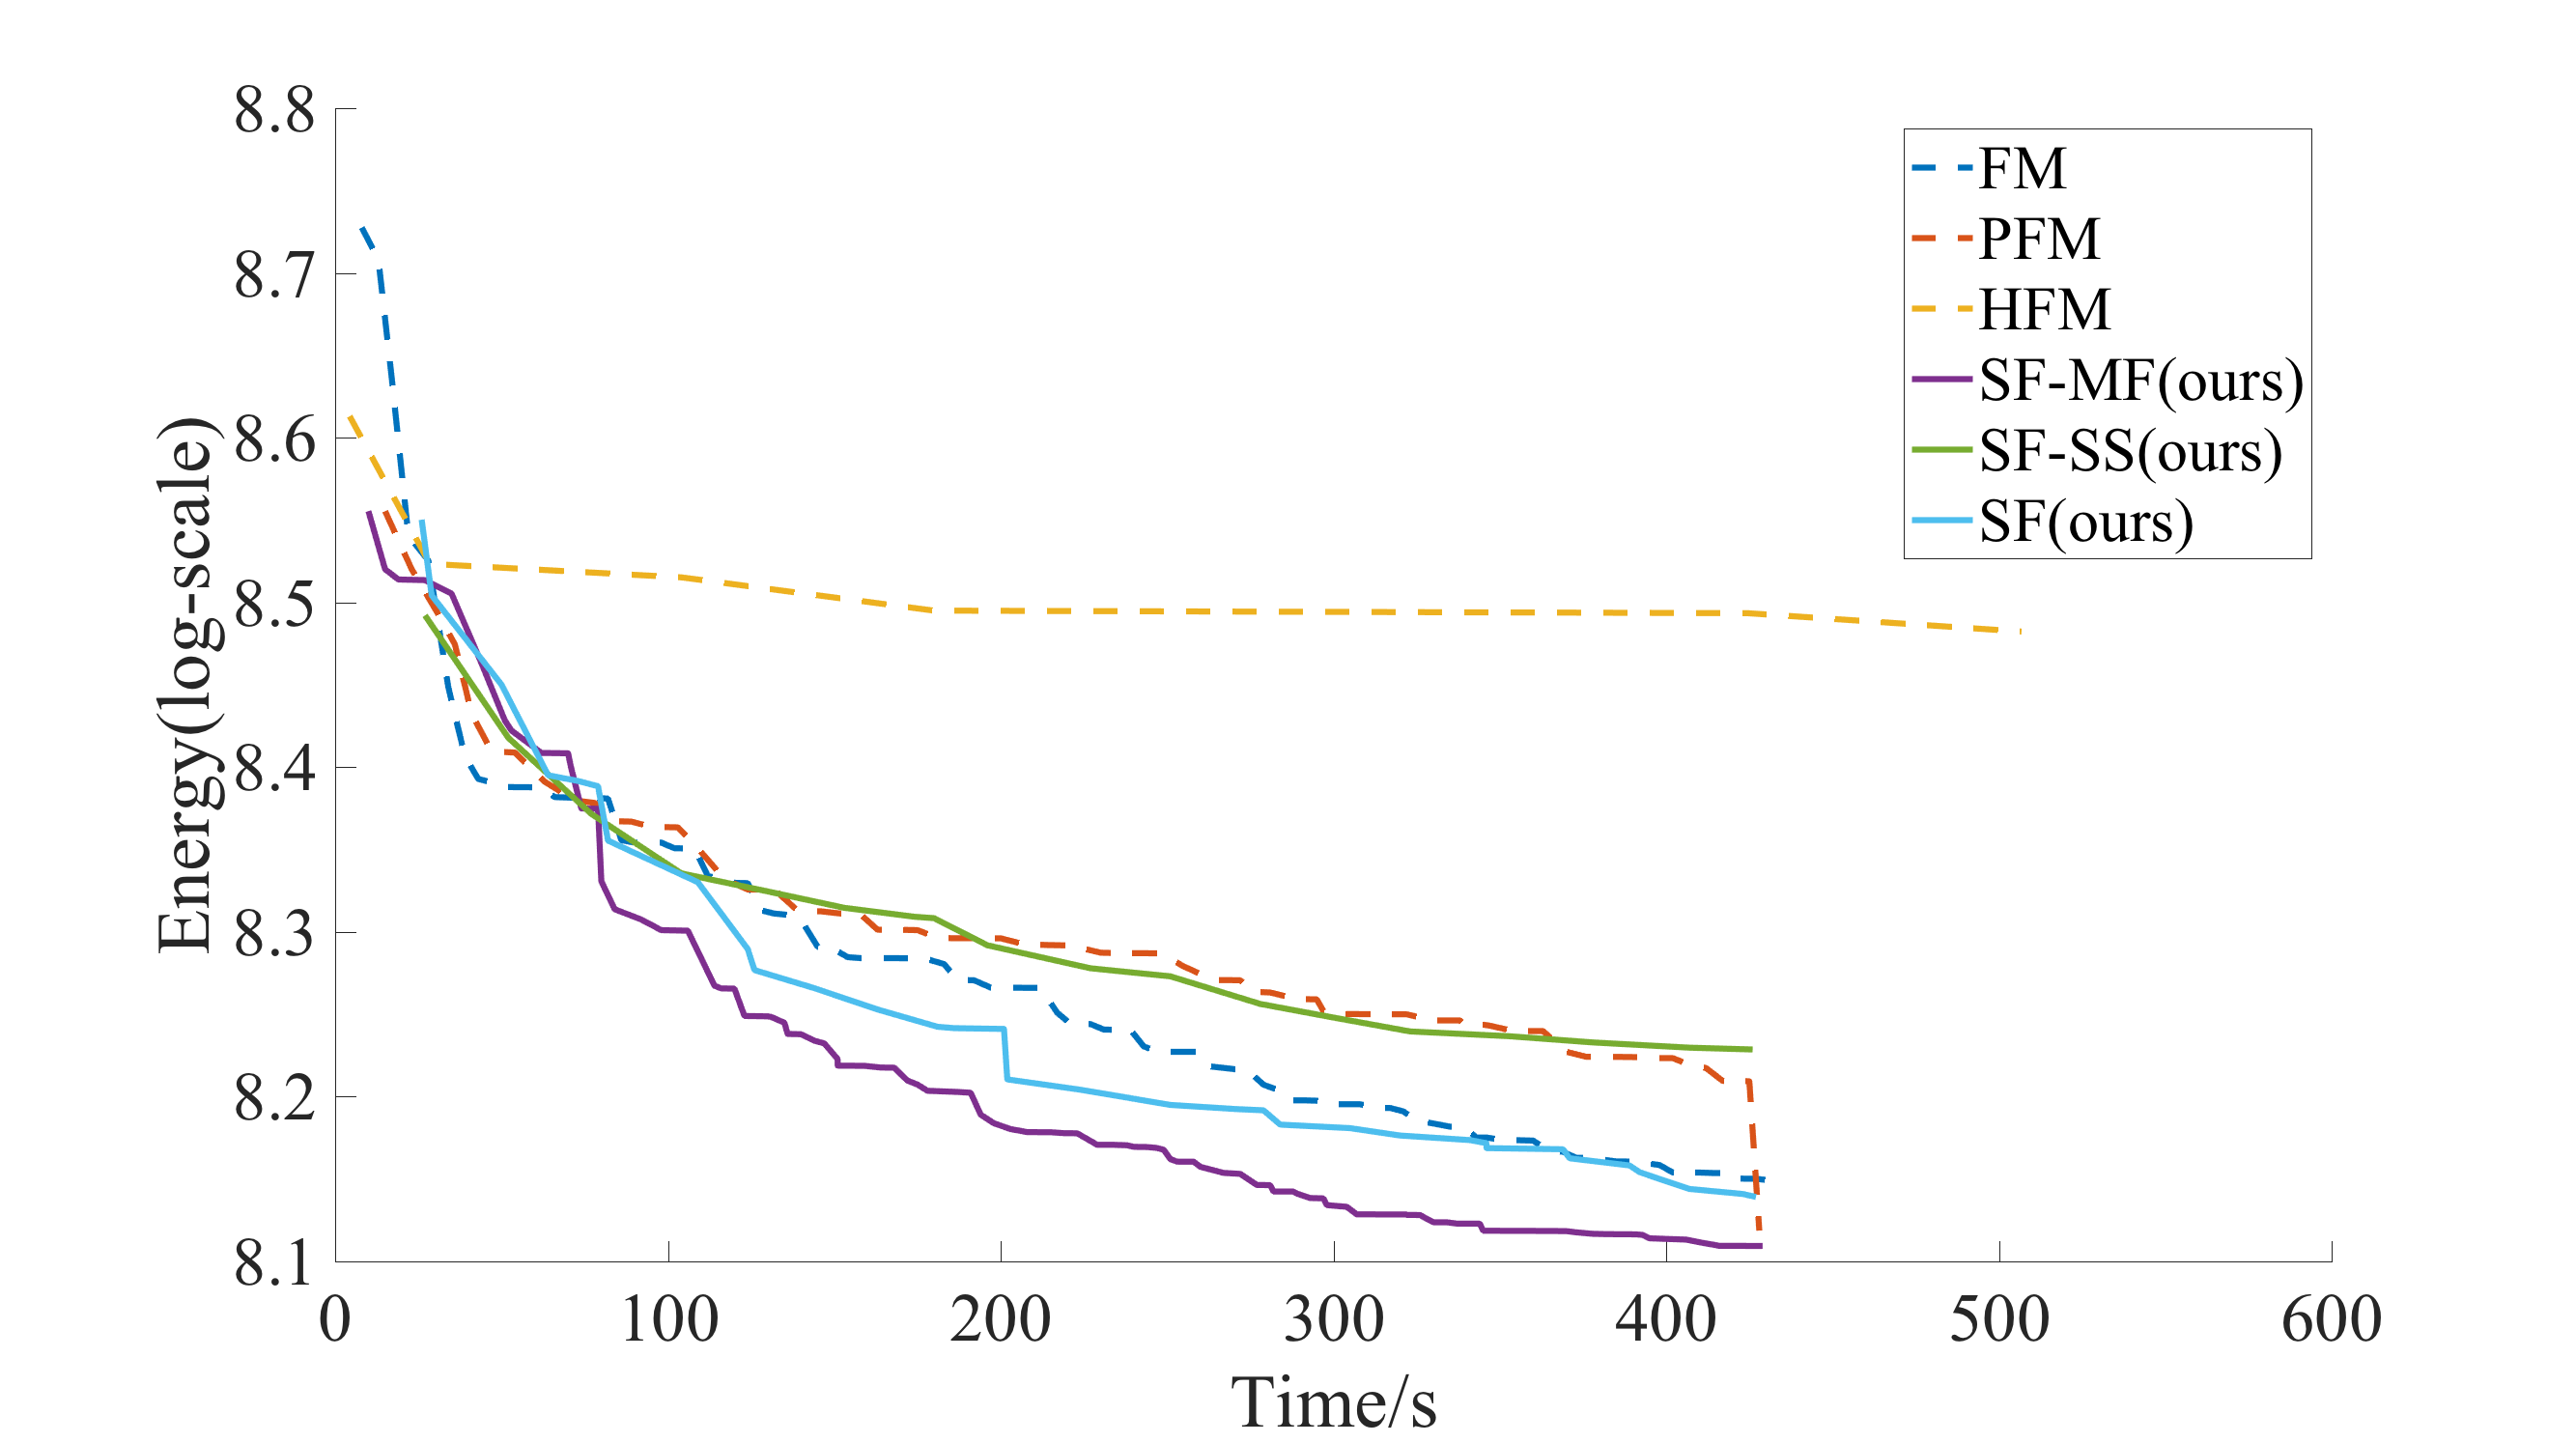
\includegraphics[width=\columnwidth]{figure/optical_flow_convergence.pdf}
  \caption{}\label{fig:optical_flow_convergence}
\end{figure}
\begin{figure}[tb]
 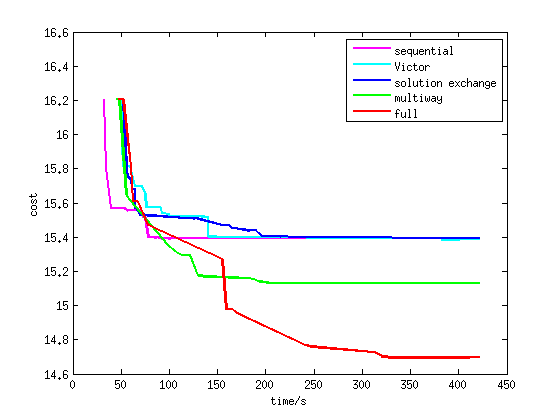
\includegraphics[width=\columnwidth]{figure/layered_depthmap_convergence.pdf}
 \caption{}\label{fig:layered_depthmap_convergence}
\end{figure}


\chen{
  From the convergence plot of layered depth map estimation, we can see that, Fusion Move, Parallel Fusion Move, and FS-MF all stalk at a high energy state. The reason is binary fusion of solution proposals (either from others or self) is too limited to further decrease the energy due to the complexity of the problem itself. Only when multi-way fusion is used (in FS-SS and FS), it becomes possible for the energy to further decrease. This coincides with the observation in \cite{layered_depthmap} that binary fusion of proposal solutions is not as powerful as their subspace fusion which is a special form of multi-way fusion here.

  As shown in \ref{section:results}, the multi-way fusion and solution sharing enabled by our uniform framework play a key role for improving performance in different settings. For better understanding our framework, we examine the role played by each factor more closely by varying each factor while keeping others the same. There are four parameters in our framework: \textit{the number of threads}, \textit{the number }
}

